% \section{Reproducibility Summary}
%
% Add your summary here. No need to worry about fitting it in a single page now.
%
% \subsection{Submission Checklist}
%
% Double check the file \texttt{journal/metadata.yaml} to contain the following information:
%
% \begin{itemize}
% \item Title should start with "\texttt{[Re]}"
% \item Author information, along with ORCID id
% \item Author affiliations
% \item Code URL, Software Heritage Foundation link
% \item Abstract
% \item Review URL (the OpenReview URL of your report)
% \end{itemize}
%
% \subsection{Continuous Integration}
%
% We use Github Actions CI to check your submission and compile the pdf file subsequently.
% You can also run the tests locally by running \texttt{python check\_yaml.py}, and then running \texttt{./build.sh} to compile Latex.
%
% \clearpage
%
% \section{Content}
% Copy your Openreview content here.
%
% This is an example citation \citep{Sinha:2021}.
% ============================================================================================================================================

% if you need to pass options to natbib, use, e.g.:
%     \PassOptionsToPackage{numbers, compress}{natbib}
% before loading neurips_2019



% to compile a preprint version, e.g., for submission to arXiv, add add the
% [preprint] option:
    % \usepackage[preprint]{neurips_2019}

% to compile a camera-ready version, add the [final] option, e.g.:
% \usepackage[final]{neurips_2019}

% to avoid loading the natbib package, add option nonatbib:
%     \usepackage[nonatbib]{neurips_2019}

% \newif{\ifhidecomments}

% The \author macro works with any number of authors. There are two commands
% used to separate the names and addresses of multiple authors: \And and \AND.
%
% Using \And between authors leaves it to LaTeX to determine where to break the
% lines. Using \AND forces a line break at that point. So, if LaTeX puts 3 of 4
% authors names on the first line, and the last on the second line, try using
% \AND instead of \And before the third author name.

\section{Reproducibility Summary}

    \subsection*{Scope of Reproducibility}
    In this paper, we work on reproducing the results obtained in the 'Fairness and Bias in Online Selection' paper \citep{correa2021fairness}. The goal of the reproduction study is to validate the 4 main claims made in \citep{correa2021fairness}. The claims made are:
    (1) for the multi-color secretary problem, an optimal online algorithm is fair, (2) for the multi-color secretary problem, an optimal offline algorithm is unfair, (3) for the multi-color prophet problem, an optimal online algorithm is fair (4) for the multi-color prophet problem, an optimal online algorithm is less efficient relative to the offline algorithm.

    To test if the results of the secretary algorithm generalize to other data sets, the proposed algorithms and baselines are applied to the UFRGS Entrance Exam and GPA data set \citep{DVN/O35FW8_2019}.
    % State the main claim(s) of the original paper you are trying to reproduce (typically the main claim(s) of the paper).
    % This is meant to place the work in context, and to tell a reader the objective of the reproduction.

    \subsection*{Methodology}
    The paper that has been reproduced includes a link to a repository containing \textit{C++} files for the algorithms that were implemented. For our experiments, we reimplemented the code in \textit{Python}. Our goal was to reproduce the code in an efficient manner without altering the core logic. Using the Python code all the experiments in the paper have been replicated including some additional experiments to verify the claims made in \citep{correa2021fairness}.

    \subsection*{Results}
    The reproduced results support all claims made in \citep{correa2021fairness}. However, in the case of the unfair secretary algorithm (SA), some irregular results arise in the experiments due to randomness. This irregularity is also existent in the original code.


    \subsection*{What was easy}
    The concepts behind the algorithms were straightforward. The existing code base provided a solid reference point to verify the results of the original paper by compiling and running the provided code.


    \subsection*{What was difficult}
    Implementing the prophet algorithm, in comparison to the secretary algorithm, was complex. \textit{C++} is a more efficient compiler (time complexity, etc.) compared to Python. For the reproduction of the algorithms, this needed to be taken into account. While it might be possible to execute transliterated code on a powerful machine, with the available resources the code would have taken over 96 hours to run. In order to tackle this problem, some of the data structures needed to be converted to \textit{NumPy} arrays to decrease computation time.


% \subsection*{Communication with original authors}
% As of now, no communication.

% Briefly describe how much contact you had with the original authors (if any).
% \newpage
% \textit{\textbf{The following section formatting is \textbf{optional}, you can also define sections as you deem fit.
% \\
% Focus on what future researchers or practitioners would find useful for reproducing or building upon the paper you choose.}}
\section{Introduction}
As more machine learning algorithms are used in decision-making circumstances, it is important to ensure that social norms are not violated. The social norm that serves as the pivot of this research is fairness. Specifically 'fairness' in the use of selection models. The importance of fairness is to avoid undesirable biases. Selection models are models that input a finite amount of agents and attempt to pick the best possible candidate (agent). The goal is to design algorithms that can fairly judge between agents regardless of any unfair bias.

% * What are online selection problems?
In some real-life implementations of selection models, there is no clear overview of all agents. For example, in the online selection problem, the agents enter the algorithm sequentially. For every agent, a decision has to be made whether this is the best possible agent. The complexity of this task is not being able to have any knowledge on agents that might come in the future. As soon as the decision is made that an agent is the best fit, the algorithm should stop as that agent is the optimal candidate (according to the model). Multiple attempts have been made to create the most accurate algorithm for these online selection models.

% * What is the secretary and the prophet problem?
For this research, we reproduce the 'Fairness and Bias in Online Selection' paper \citep{correa2021fairness}. In this paper, the authors focus on 2 main problems: the secretary problem and the prophet problem. The secretary problem is a scenario for the sequential selection problem where an attempt is made to select the candidate with the highest value without knowing the value of the candidates to come. An immediate decision has to be made on the candidate, the candidate either gets picked or gets passed on. For the prophet algorithm the same assumptions are made as for the secretary algorithm, but we know the distributions the candidate values are drawn from. The probability of the candidate is based on these distributions. In the case of both problems, the goal is to stop at the best possible candidate based on the assigned probabilities.

% * How is fairness defined in context of the online selection problem?
In order to include a form of fairness in these models, a concrete definition needs to be given to fairness in online selection models. Based on the \citep{correa2021fairness} paper, fairness is defined as an unbiased evaluation of agents in a selection model. A selection algorithm is fair if it selects the best candidate, closely following the original probability of the best candidate existing in that group. Along with fairness, efficiency has also been used as an evaluation metric in the original paper. Efficiency is a measure of how accurately the online algorithm picks the actual best candidate.

By creating a 'fair' version for these problems, the authors claim to have created a fair use of sequential single item selection models. Through categorization of the agents by color, a distinction between the agents can be made. However, the qualities these agents possess might be different enough that they could be considered incomparable. So implementing a multi-color version of the sequential selection models and picking the best possible candidate, taking color into account, an 'unfair' comparison is avoided.

\section{Scope of reproducibility}
\label{sec:claims}
In this reproduction study, we focus on the authors' claims that the use of a multi-color version of the secretary and prophet problem would make the use of these algorithms fair. The authors of the paper implement these algorithms on synthetic data sets and real-world data sets.

For our study, we put an effort into reproducing the results given by the paper. The goal of this reproduction is to either validate or deny the claims made in the paper. This effort has been fulfilled by re-implementing the code publicly available for the algorithm. This re-implementation is done in \textit{Python} in comparison to the \textit{C++} code provided by the authors. Most of the code has been written using \textit{NumPy} to try and achieve about the same efficiency as the \textit{C++} code. However, the setup for the experiments corresponds to that of the authors.

To show that the claims generalize well over differently distributed data sets, we run the proposed algorithms and baselines on the UFRGS Entrance Exam and GPA data set \citep{DVN/O35FW8_2019}.

% Introduce the specific setting or problem addressed in this work, and list the main claims from the original paper. Think of this as writing out the main contributions of the original paper. Each claim should be relatively concise; some papers may not clearly list their claims, and one must formulate them in terms of the presented experiments. (For those familiar, these claims are roughly the scientific hypotheses evaluated in the original work.)


% A claim should be something that can be supported or rejected by your data. An example is, ``Finetuning pretrained BERT on data set X will have higher accuracy than an LSTM trained with GloVe embeddings.''
% This is concise, and is something that can be supported by experiments.
% An example of a claim that is too vague, which can't be supported by experiments, is ``Contextual embedding models have shown strong performance on a number of tasks. We will run experiments evaluating two types of contextual embedding models on data sets X, Y, and Z."

% This section roughly tells a reader what to expect in the rest of the report. Clearly itemize the claims you are testing:
The claims made in the \citep{correa2021fairness} paper are:
\begin{itemize}
  \item Claim 1: For the multi-color secretary problem, an optimal online algorithm is fair. \label{claim1}
  \item Claim 2: For the multi-color secretary problem, an optimal offline algorithm is unfair.
  \label{claim2}
  \item Claim 3: For the multi-color prophet problem, an optimal online algorithm is fair.
  \item Claim 4: For the multi-color prophet problem, an optimal online algorithm is less efficient relative to the offline algorithm.
\end{itemize}

To test these claims we use the algorithms mentioned above on 4 types of data sets. These data sets are further discussed in section 3.3.

% Each experiment in Section~\ref{sec:results} will support (at least) one of these claims, so a reader of your report should be able to separately understand the \emph{claims} and the \emph{evidence} that supports them.

%\jdcomment{To organizers: I asked my students to connect the main claims and the experiments that supported them. For example, in this list above they could have ``Claim 1, which is supported by Experiment 1 in Figure 1.'' The benefit was that this caused the students to think about what their experiments were showing (as opposed to blindly rerunning each experiment and not considering how it fit into the overall story), but honestly it seemed hard for the students to understand what I was asking for.}
% \newpage
\section{Methodology}\label{meth}
In this section, our approach to the re-implementation of the experiments will be discussed and an additional experiment will be proposed.
% Explain your approach - did you use the author's code, or did you aim to re-implement the approach ferom the description in the paper? Summarize the resources (code, documentation, GPUs) that you used.

\subsection{Code}
The code accompanying the paper is provided in \textit{C++}. As required for this study, we reproduced the work in Python, and subsequently made use of the inherent Pythonic efficiencies. The provided code allowed for a smooth initial reproduction. However, many optimisations were required to decrease computation duration.

\subsection{Model descriptions}
In the original paper, two types of single item selection models are considered: the secretary algorithm and the prophet algorithm. Candidates are partitioned into different groups which the authors refer to as \textit{colors}. Every candidate has a numerical value that indicates the capabilities of that candidate. The authors refer to these indicators as \textit{values}. Candidates arrive sequentially, and upon arrival, the algorithms decide whether the candidate is the best candidate overall. The best candidate is defined as the candidate with the highest value of the sequence of candidates. For clarity, the main parts of the Methodology and Results sections are divided per model.

\subsubsection{Secretary Algorithm}
For the secretary algorithm, it is assumed that candidates arrive in uniformly random order. To verify the claims made by the author, we compare the optimal online algorithm as proposed by \citep{correa2021fairness} to two baselines. Additionally, the algorithm and its baselines are applied on different data sets, either synthetically generated or composed from real-word data sets. The optimal online algorithm proposed by the authors (Fair secretary algorithm) is denoted formally as:
\begin{figure}[H]
    \centering
    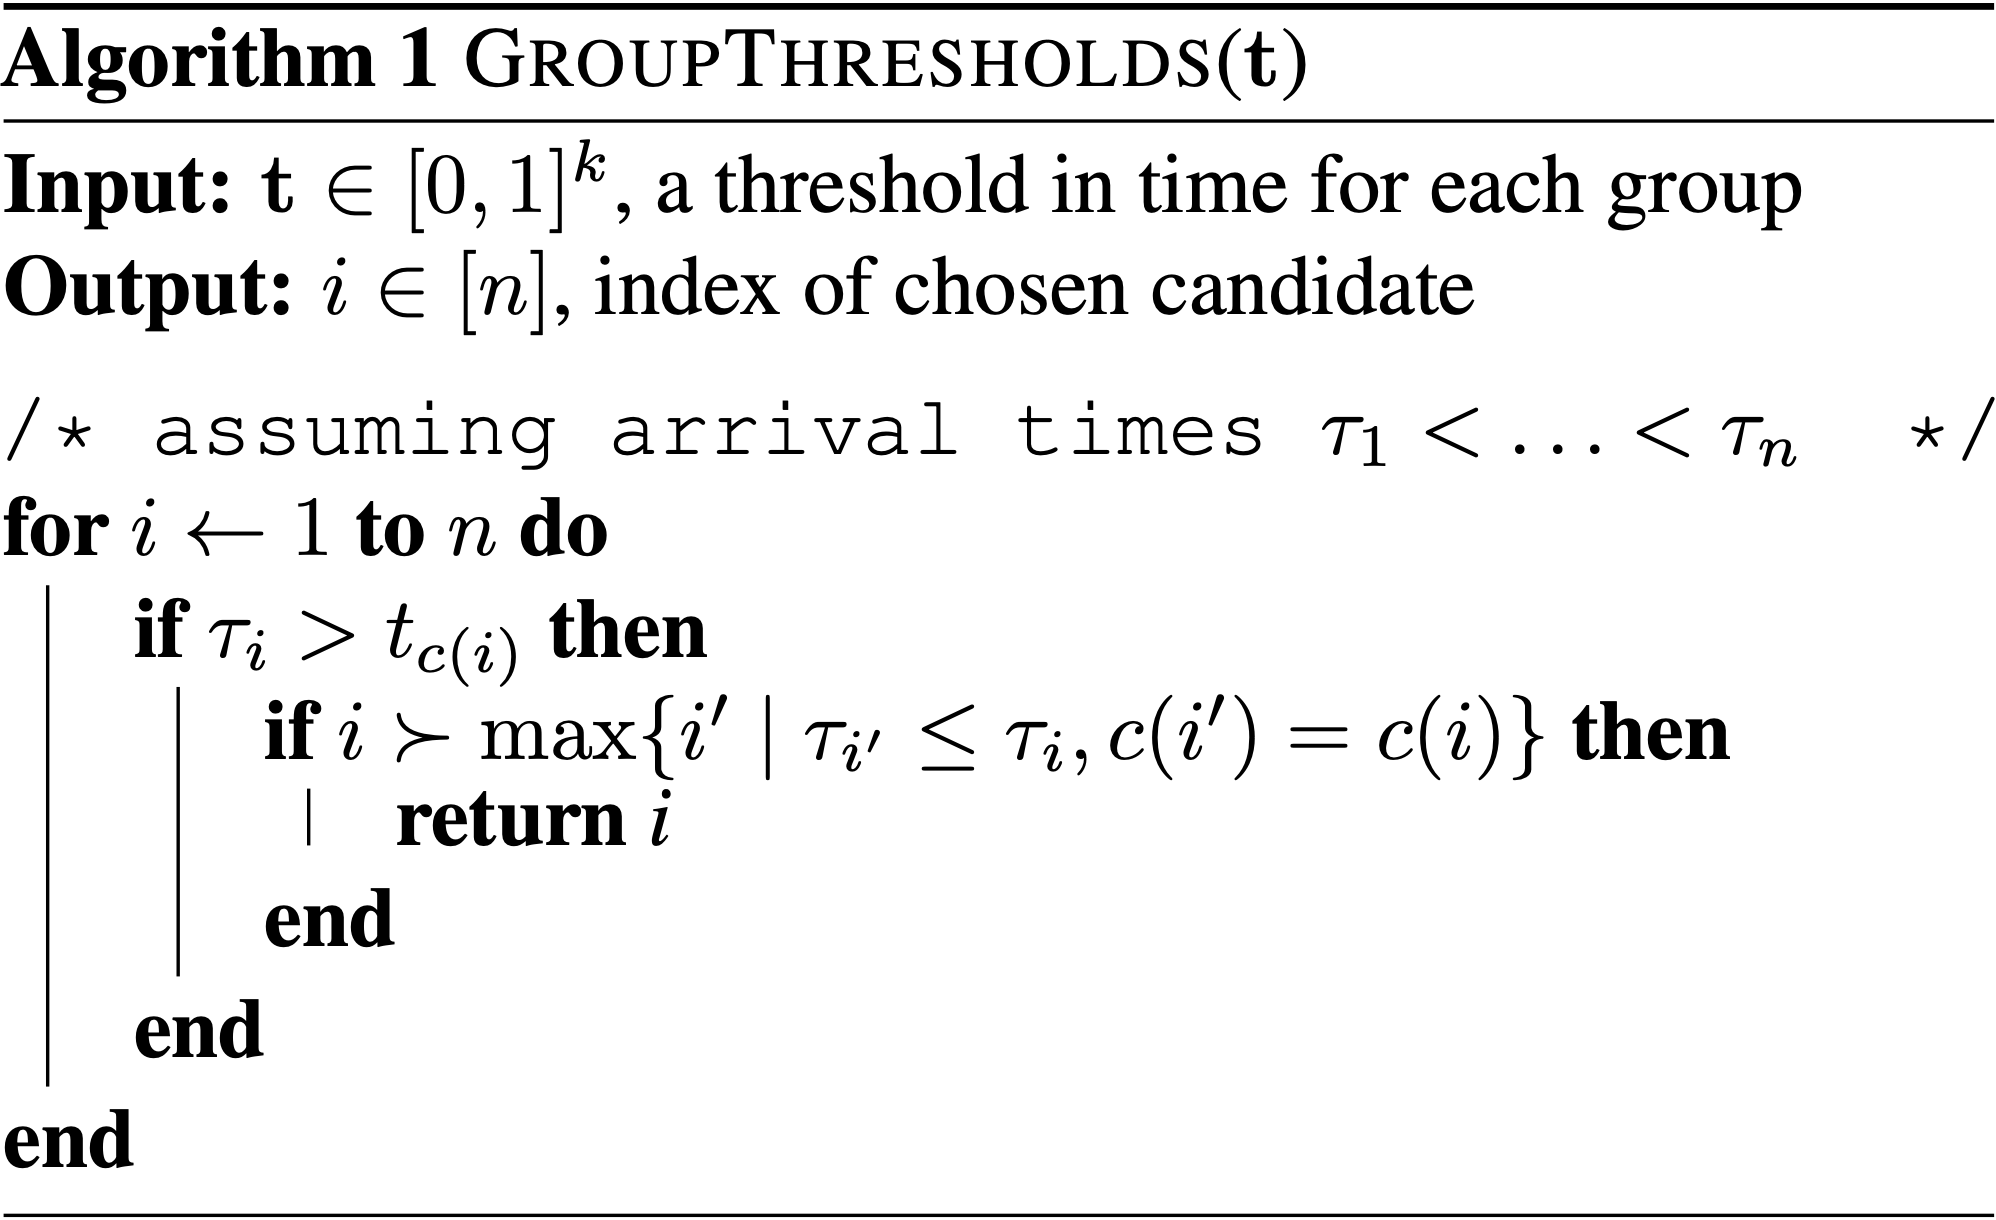
\includegraphics[width=0.5\linewidth]{media/algosa.png}
    \label{fig:algosa}
\end{figure}
% \begin{algorithm}
% \caption{GroupThresholds(t)}
% \begin{algorithmic}
% \KwInput{\mathbf{t} \in[0,1]^{k}, a threshold in time for each group}
%  \KwOutput{i \in[n], index of chosen candidate }
% \end{algorithmic}
% \end{algorithm}

where the input \textbf{t} $= (t_1, ..., t_k)$ is a vector of thresholds, one for each color $j \in [k]$. The algorithm first checks if the candidate $i$ arrived after the threshold of its color $t_{c(i)}$. If this condition is met, it accepts the candidate if its value exceeds the value of all previous candidates of color $t_{c(i)}$, indicating that it is the best candidate for that color.

After having chosen the best candidate of each color, we are interested in selecting the best overall candidate. We denote the probabilities with which the best candidate of group $j$ is the best among all colors by $p_j$, which results in the vector \textbf{p} $= (p_1,...,p_k)$ covering all colors. We use this in our experiments to verify the claims of the author using equal, and unequal values for \textbf{p} among colors.

\subsubsection{Prophet Algorithm}
For the prophet algorithm, the same assumptions are made as for the secretary algorithm, but we know the distributions $F_i$ the candidate values are drawn from. In the paper, the authors propose two optimal online algorithms specified in figure \ref{fig:prophetalgos}, where $q_1, \cdots, q_n$ denote the marginal probabilities that the optimal fair offline algorithm picks the candidates $i=1, \cdots, n$. Figure \ref{fig:genpro} shows the general Fair prophet algorithm (Fair prophet algorithm). This algorithm does not make any assumptions about the underlying probability distribution, it can be different for every candidate. Figure \ref{fig:iidpro} shows the Fair independent and identically distributed prophet algorithm (Fair IID prophet algorithm). This algorithm assumes that the values of the candidates are drawn from the same distribution.

\begin{figure*}[h!]
    \centering
    \begin{subfigure}[t!]{0.475\textwidth}
         \centering
        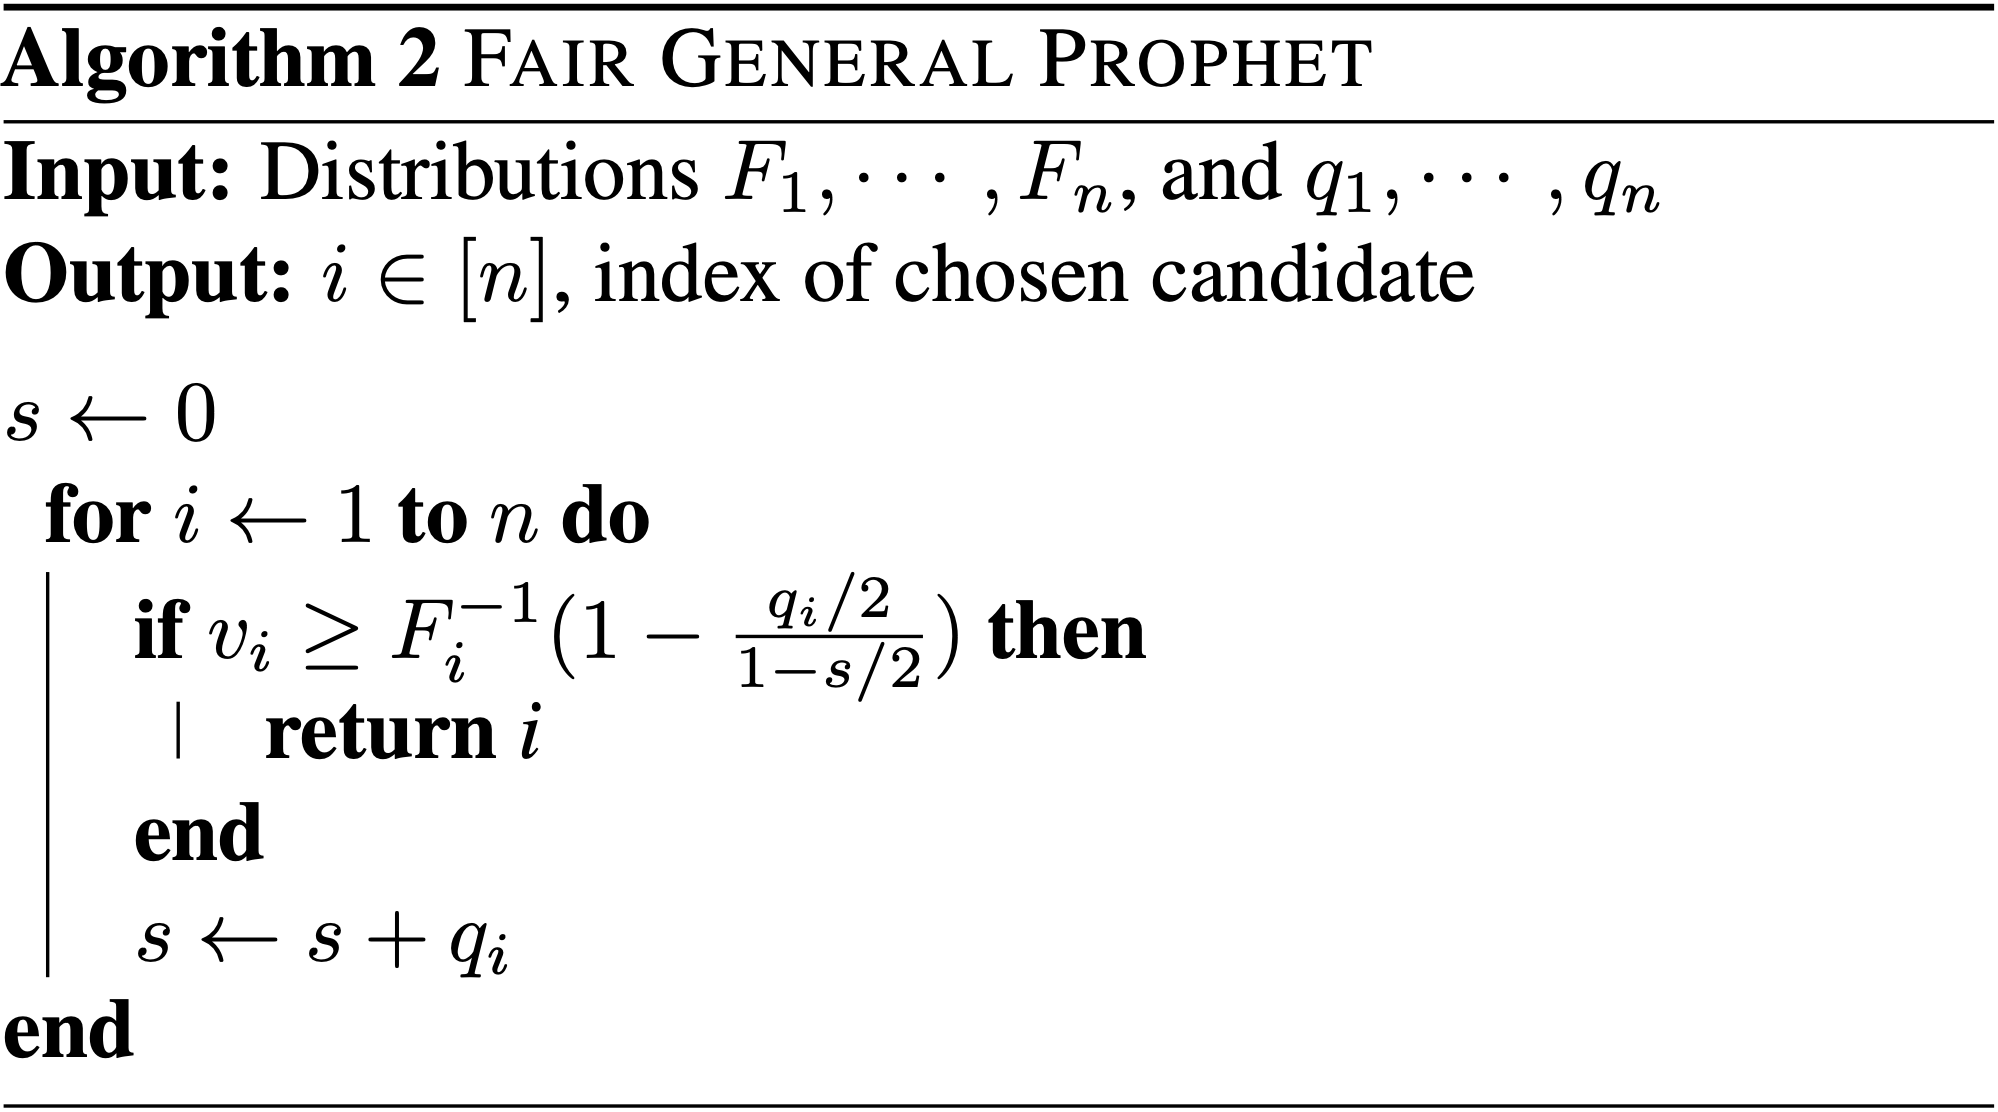
\includegraphics[width=1\textwidth]{media/generalpro.png}
        \caption{Fair prophet algorithm}
        \label{fig:genpro}
    \end{subfigure}
    \hfill
    \begin{subfigure}[t!]{0.475\textwidth}
        \centering
        \includegraphics[width=1\textwidth]{media/iddpro.png}
        \caption{Fair IID prophet algorithm}
        \label{fig:iidpro}
    \end{subfigure}
    \caption{Fair prophet algorithms proposed by the authors.}
    \label{fig:prophetalgos}
\end{figure*}

% Include a description of each model or algorithm used. Be sure to list the type of model, the number of parameters, and other relevant info (e.g. if it's pretrained).

\subsection{Data sets}
% For each data set include 1) relevant statistics such as the number of examples and label distributions, 2) details of train / dev / test splits, 3) an explanation of any preprocessing done, and 4) a link to download the data (if available).
The experiments involving the SA algorithm are conducted on two synthetic data sets and two real-world data sets. The data sets and their properties are summarised below:

\begin{enumerate}
    \item \textbf{Synthetic data set, equal p values} contains four different colors with 10, 100, 1000, and 10000 occurrences. The value of each element is chosen independently and uniformly at random from [0, 1]. \label{equalp}
    \item \textbf{Synthetic data set, general p values} contains a similar setup as \ref{equalp}, but with \textit{p} $= (0.3, 0.25, 0.25, 0.2)$.
    \item \textbf{Feedback maximization (Bank)} contains records of direct marketing campaigns (phone calls) by a Portuguese banking institution \citep{bankport}. The clients are split into 5 colors by age: under 30, 31-40, 41-50, 51-60, and over 61 years old. The value of every client is the duration of the phone call. Moreover, an equal \textit{p} of 0.2 was used for all colors.

    \item \textbf{Influence maximization (Pokec)} contains records of the influence of users of the Pokec social network \citep{pokec}. We pre-process the data by dividing the users into 5 different colors according to their body mass index (BMI): under weighted (BMI < 18.5), normal (18.5 <= BMI < 25), over weighted (25.0 <= BMI < 30.0), obese type 1 (30.0 <= BMI < 35), and obese type 2 (BMI >= 35.0). The value is computed as the number of the followers for each user. Again, an equal \textit{p} of 0.2 was used for all colors.
    \end{enumerate}

\subsection{Experimental setup}
\label{experimental_setup}
% Include a description of how the experiments were set up that's clear enough a reader could replicate the setup.
% Include a description of the specific measure used to evaluate the experiments (e.g. accuracy, precision@K, BLEU score, etc.).
% Provide a link to your code.
In this subsection, the experimental evaluation performed by the authors is discussed. As before, a distinction between the two problems is made for clarity. Additionally, an extra experiment will be considered where the secretary algorithm will be evaluated on another real-world data set. \\
% \newpage
\textbf{Secretary experiments}
\FloatBarrier
\label{Secretary_Experiments}
The authors propose two different baselines to compare the Fair secretary algorithm to. Firstly, the classic secretary algorithm (SA), which does not take the colors of the candidates into account. Secondly, the single-color secretary algorithm (SCSA). This algorithm picks a color proportional to the \textit{p} values and then runs the classic secretary algorithm on the candidates of only that color. To evaluate the claims by the authors, the three mentioned algorithms are evaluated against the four data sets discussed earlier.

The parameters of these experiments consist of the size of the data sets and the number of repetitions. For the experiments on the Synthetic data sets (equal \textit{p} / general \textit{p}) and the Bank data set, all available candidates were used in 20.000 repetitions. In the original paper, the authors used all $\pm$ 650.000 candidates of the Pokec data set in 1000.000 repetitions. In our experiment, we had to limit these parameters due to time constraints. We only considered the first 40.000 candidates and used 40.000 repetitions.\\

% \newpage
\textbf{Prophet experiments}
\FloatBarrier
\label{Prophet_Experiments}
For the prophet experiments, the Fair prophet algorithm and Fair IID prophet algorithm are evaluated against three baselines: the SC algorithm \citep{samuel1984comparison}, EHKS algorithm \citep{marx2021proceedings}, CFHOV algorithm \citep{correa2021posted} and DP algorithm \citep{brown1972great}. The specific works of these algorithms are described in further detail in the paper \citep{correa2021fairness} section 4.2.

For the experiments, two settings are implemented. In the first setting, 50 samples are taken from a uniform distribution in a range of [0, 1]. These samples function as the input stream. In the second setting, 1000 samples are taken from a binomial distribution with 1000 trials and a probability of a successful single trial $p = 0.5$. In order to compare this method with the already existing algorithms, we assume each candidate to be group of its own. For every algorithm, we repeat the experiment 50.000 times.\\

\textbf{Extending to other data set (UFRGS) experiments}
\FloatBarrier
\label{Work_beyond_original_paper}
This subsection describes an experimental extension on the work of \citep{correa2021fairness}. In our work, we have concluded that the secretary results claimed in the paper are reproducible. It is shown in section \ref{results_reproducting_original_paper} that the Fair algorithm significantly outperforms the SCSA baseline. However, all real-world data sets used to prove this claim contain the same distribution of values for every color. The distributions for the Bank and Pokec data sets are shown in Figures \ref{distribution_bank} \ref{distribution_pokec} respectively.

Our extension investigates the effect of applying the Fair algorithm to an unequally distributed real-word data set, such as the UFRGS Entrance Exam and GPA Data (UFRGS) data set. This work will show whether the claims made by the authors generalize to these types of data sets. The UFRGS contains entrance exam scores of students applying to a university in Brazil (Federal University of Rio Grande do Sul), along with the students' GPAs during the first three semesters at university. The data set also includes the gender of every student (male or female).
The distribution of the data set is shown in Figure \ref{distribution_ufrgs}. This experiment is a duplication of the original secretary experiments but with the UFRGS data set as input. The gender of the students is used as color, their GPA score as values. The experiment is repeated 20.000 times.

\begin{figure*}[h!]
    \centering
    \begin{subfigure}[t]{0.32\textwidth}
         \centering
        \includegraphics[width=1\textwidth]{media/Images_plots/dataset_distribution_Bank.png}
        \caption{Bank data set}
        \label{distribution_bank}
    \end{subfigure}
    \hfill
    \begin{subfigure}[t]{0.32\textwidth}
        \centering
        \includegraphics[width=1\textwidth]{media/Images_plots/dataset_distribution_Pokec.png}
        \caption{Pokec data set}
        \label{distribution_pokec}
    \end{subfigure}
    \begin{subfigure}[t]{0.32\textwidth}
        \centering
        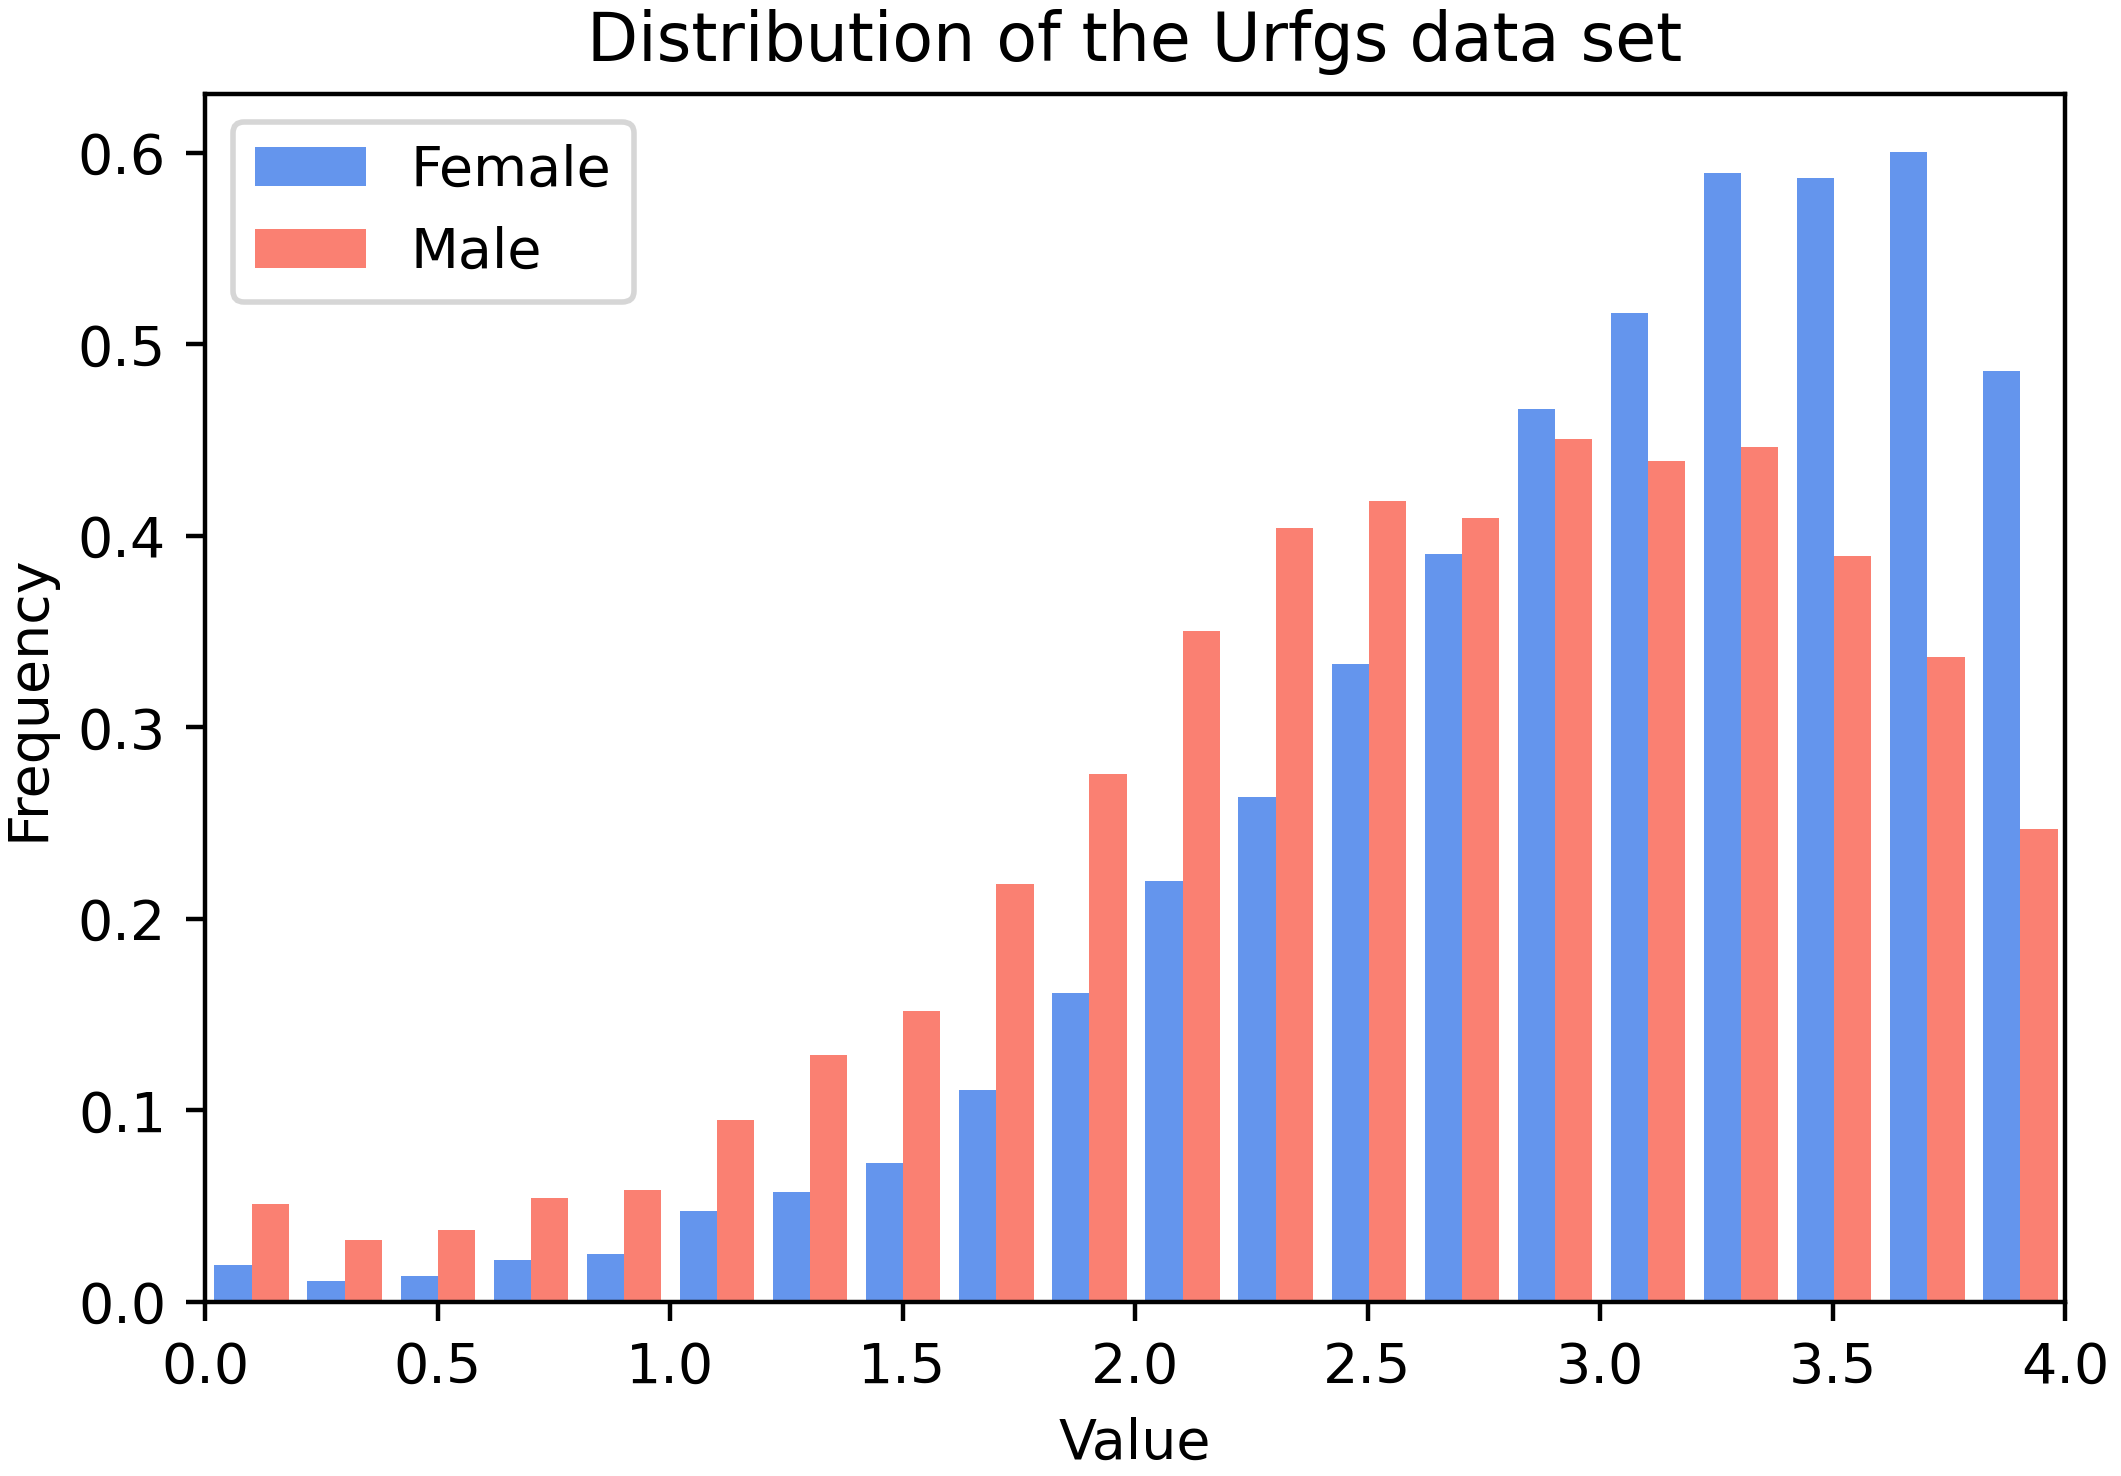
\includegraphics[width=1\textwidth]{media/Images_plots/dataset_distribution_Urfgs.png}
        \caption{Urfgs data set}
        \label{distribution_ufrgs}
    \end{subfigure}
    \caption{Value distributions of the different color groups in the real-world secretary algorithm data sets.}
    \label{fig:distributions}
\end{figure*}

% \subsection{Computational requirements}
% Include a description of the hardware used, such as the GPU or CPU the experiments were run on.
% For each model, include a measure of the average runtime (e.g. average time to predict labels for a given validation set with a particular batch size).
% For each experiment, include the total computational requirements (e.g. the total GPU hours spent).
% (Note: you'll likely have to record this as you run your experiments, so it's better to think about it ahead of time). Generally, consider the perspective of a reader who wants to use the approach described in the paper --- list what they would find useful.
% , , ,

\section{Results}
\label{sec:results}
The following paragraphs will present the results for the experiments discussed in section \ref{experimental_setup}: (1) the secretary experiments, (2) the prophet experiments, (3) our extended work. \\
% [TODO]For each experiment, say 1) which claim in Section~\ref{sec:claims} it supports, and 2) if it successfully reproduced the associated experiment in the original paper.
% For example, an experiment training and evaluating a model on a data set may support a claim that that model outperforms some baseline.
% Logically group related results into sections.

\textbf{Secretary results}
\FloatBarrier
The plots in Figure \ref{fig:sa_plots} show our reproduction work regarding the original paper on the secretary problem over the four different data sets. We find that all results are in line with the work of \citep{correa2021fairness}. Due to the nature of construction of the fair algorithm proposed by the authors, and the SCSA, we find that it picks elements from each color proportional to the vector \textbf{p}. From this, it can be concluded that the authors' Claims 1 and 2 are valid.

% , and therefore conclude that based on this section's experiments Claim \ref{claim1}, and Claim \ref{claim2} are reproducible.

\begin{figure*}[h!]
    \centering
    \begin{subfigure}[b]{0.475\textwidth}
        \centering
        \includegraphics[width=\textwidth]{media/Images_plots/Secretaryplot_equal__ (1).png}
        \caption[Network2]%
        {{\small Synthetic Data set Equal \textit{p}}}
        \label{fig:mean and std of net14}
    \end{subfigure}
    \hfill
    \begin{subfigure}[b]{0.475\textwidth}
        \centering
        \includegraphics[width=\textwidth]{media/Images_plots/Secretaryplot_general__.png}
        \caption[]%
        {{\small Synthetic Data set General \textit{p}}}
        \label{fig:mean and std of net24}
    \end{subfigure}
    \vskip\baselineskip
    \begin{subfigure}[b]{0.475\textwidth}
        \centering
        \includegraphics[width=\textwidth]{media/Images_plots/Secretaryplot_bank__.png}
        \caption[]%
        {{\small Feedback Maximization}}
        \label{fig:mean and std of net34}
    \end{subfigure}
    \hfill
    \begin{subfigure}[b]{0.475\textwidth}
        \centering
        \includegraphics[width=\textwidth]{media/Images_plots/Secretaryplot_pokec__.png}
        \caption[]%
        {{\small Influence Maximization}}
        \label{fig:mean and std of net44}
    \end{subfigure}
    \caption[]
    {\small Reproduction work regarding the original paper on the secretary problem. Comparing the Fair secretary algorithm to the aforementioned baselines SA, SCSA over four different data sets: (a) synthetic data set, equal \textit{p} values, (b) synthetic data set, general \textit{p} values, (c) feedback maximization data set (Bank), and (d) influence maximization data set (Pokec). Input denotes the number of elements from each color in the input, F-Pick and F-Max are the number of elements picked by the fair secretary algorithm and the number of them that are the maximum among the elements of that color. Similarly, U-Pick (S-Pick) and U-Max (S-Max) are the number of elements picked by SA and SCSA and the number of them that are the maximum among the elements of that color }
    \label{fig:sa_plots}
\end{figure*}

The authors claim that the quality of the solution of their algorithm is significantly higher than the SCSA. Table \ref{tab:secretary} shows our replication of this comparison. We find that our implementation reproduces the authors' claim that their method is superior to the SCSA. Small discrepancies in the results are found, this is due to the random nature of the algorithm. However, as mentioned earlier, after scrutinizing the distributions of the used data sets, we found that all the used data sets have similar distributions in the input. Therefore, we proceed by agreeing with the claims of the author given this restriction.

\begin{table}[h]
\centering
\resizebox{\columnwidth}{!}{
\begin{tabular}{lllll}
\hline
Data set & Claimed Pick & Reproduction Pick & Claimed Max & Reproduction Max \\
\hline
Synthetic (Equal \textit{p})   & 1.305 (+30.5\%) & 1.326 (+32.6\%) & 1.721 (+73.1\%) & 1.685 (+68.5\%)  \\
Synthetic (General \textit{p}) & 1.309 (+30.9\%) & 1.334 (+33.4\%) & 1.630 (+63.0\%) & 1.666 (+66.6\%)  \\
Bank & 1.347 (+34.7\%) & 1.377 (+37.7\%) & 1.760 (+76.0\%) & 1.812 (+81.2\%) \\
Pokec & 1.373 (+37.3\%) & 1.368 (+36.8\%) & 1.756 (+75.6\%) & 1.810 (+81.0\%) \\
UFGRS & - & 1.192 (+19.2\%) & - & 1.364 (+36.4\%)  \\
\hline
\end{tabular}
}
\caption{Secretary experiment claims by the author compared to reproduced results.}
\label{tab:secretary}
\end{table}

% \newpage

\textbf{Prophet results}
\FloatBarrier
The patterns of the results in the original paper are reflected in our reproduction as visualized in figured \ref{fig:propresults}. A major difference is that the scale of their y-axis is twice the size of our reproduction. Because the shown plots are a histogram of arrival positions, this could be attributed to a difference in bin size. The authors' report specifies using uniform distributions. Table \ref{tab:prophet} shows our replication of the average values chosen by each algorithm. While small differences exist, our reproduction mirrors the authors' results upon running their code closely.
\begin{table}[h]
\centering
\resizebox{\columnwidth}{!}{
\begin{tabular}{lllll}
\hline
& \multicolumn{2}{l}{Uniform Distribution}& \multicolumn{2}{l}{Binomial Distribution}\\
\hline
Algorithm & Claimed value & Reproduction value & Claimed value & Reproduction value \\
\hline
Fair PA & 0.501 & 0.497 & 0.297 & 0.273 \\
Fair IID & 0.661 & 0.654 & 0.389 & 0.364 \\
SC & 0.499 & 0.494 & 0.227 & 0.253\\
EHKS & 0.631 & 0.625 & 0.362 & 0.339\\
CFHOV & 0.752 & 0.755 & 0.513 & 0.408\\
DP & 0.751 & 0.752 & 0.429 & 0.340\\
\hline
\end{tabular}
}
\caption{Prophet experiment claims by the author compared to reproduced results.}
\label{tab:prophet}
\end{table}
% Despite the deviations caused by a difference in bin size, it can be concluded that the authors' Claims 3 and 4 are valid.

\begin{figure*}[h!]
    \centering
    \begin{subfigure}[b]{0.475\textwidth}
         \centering
        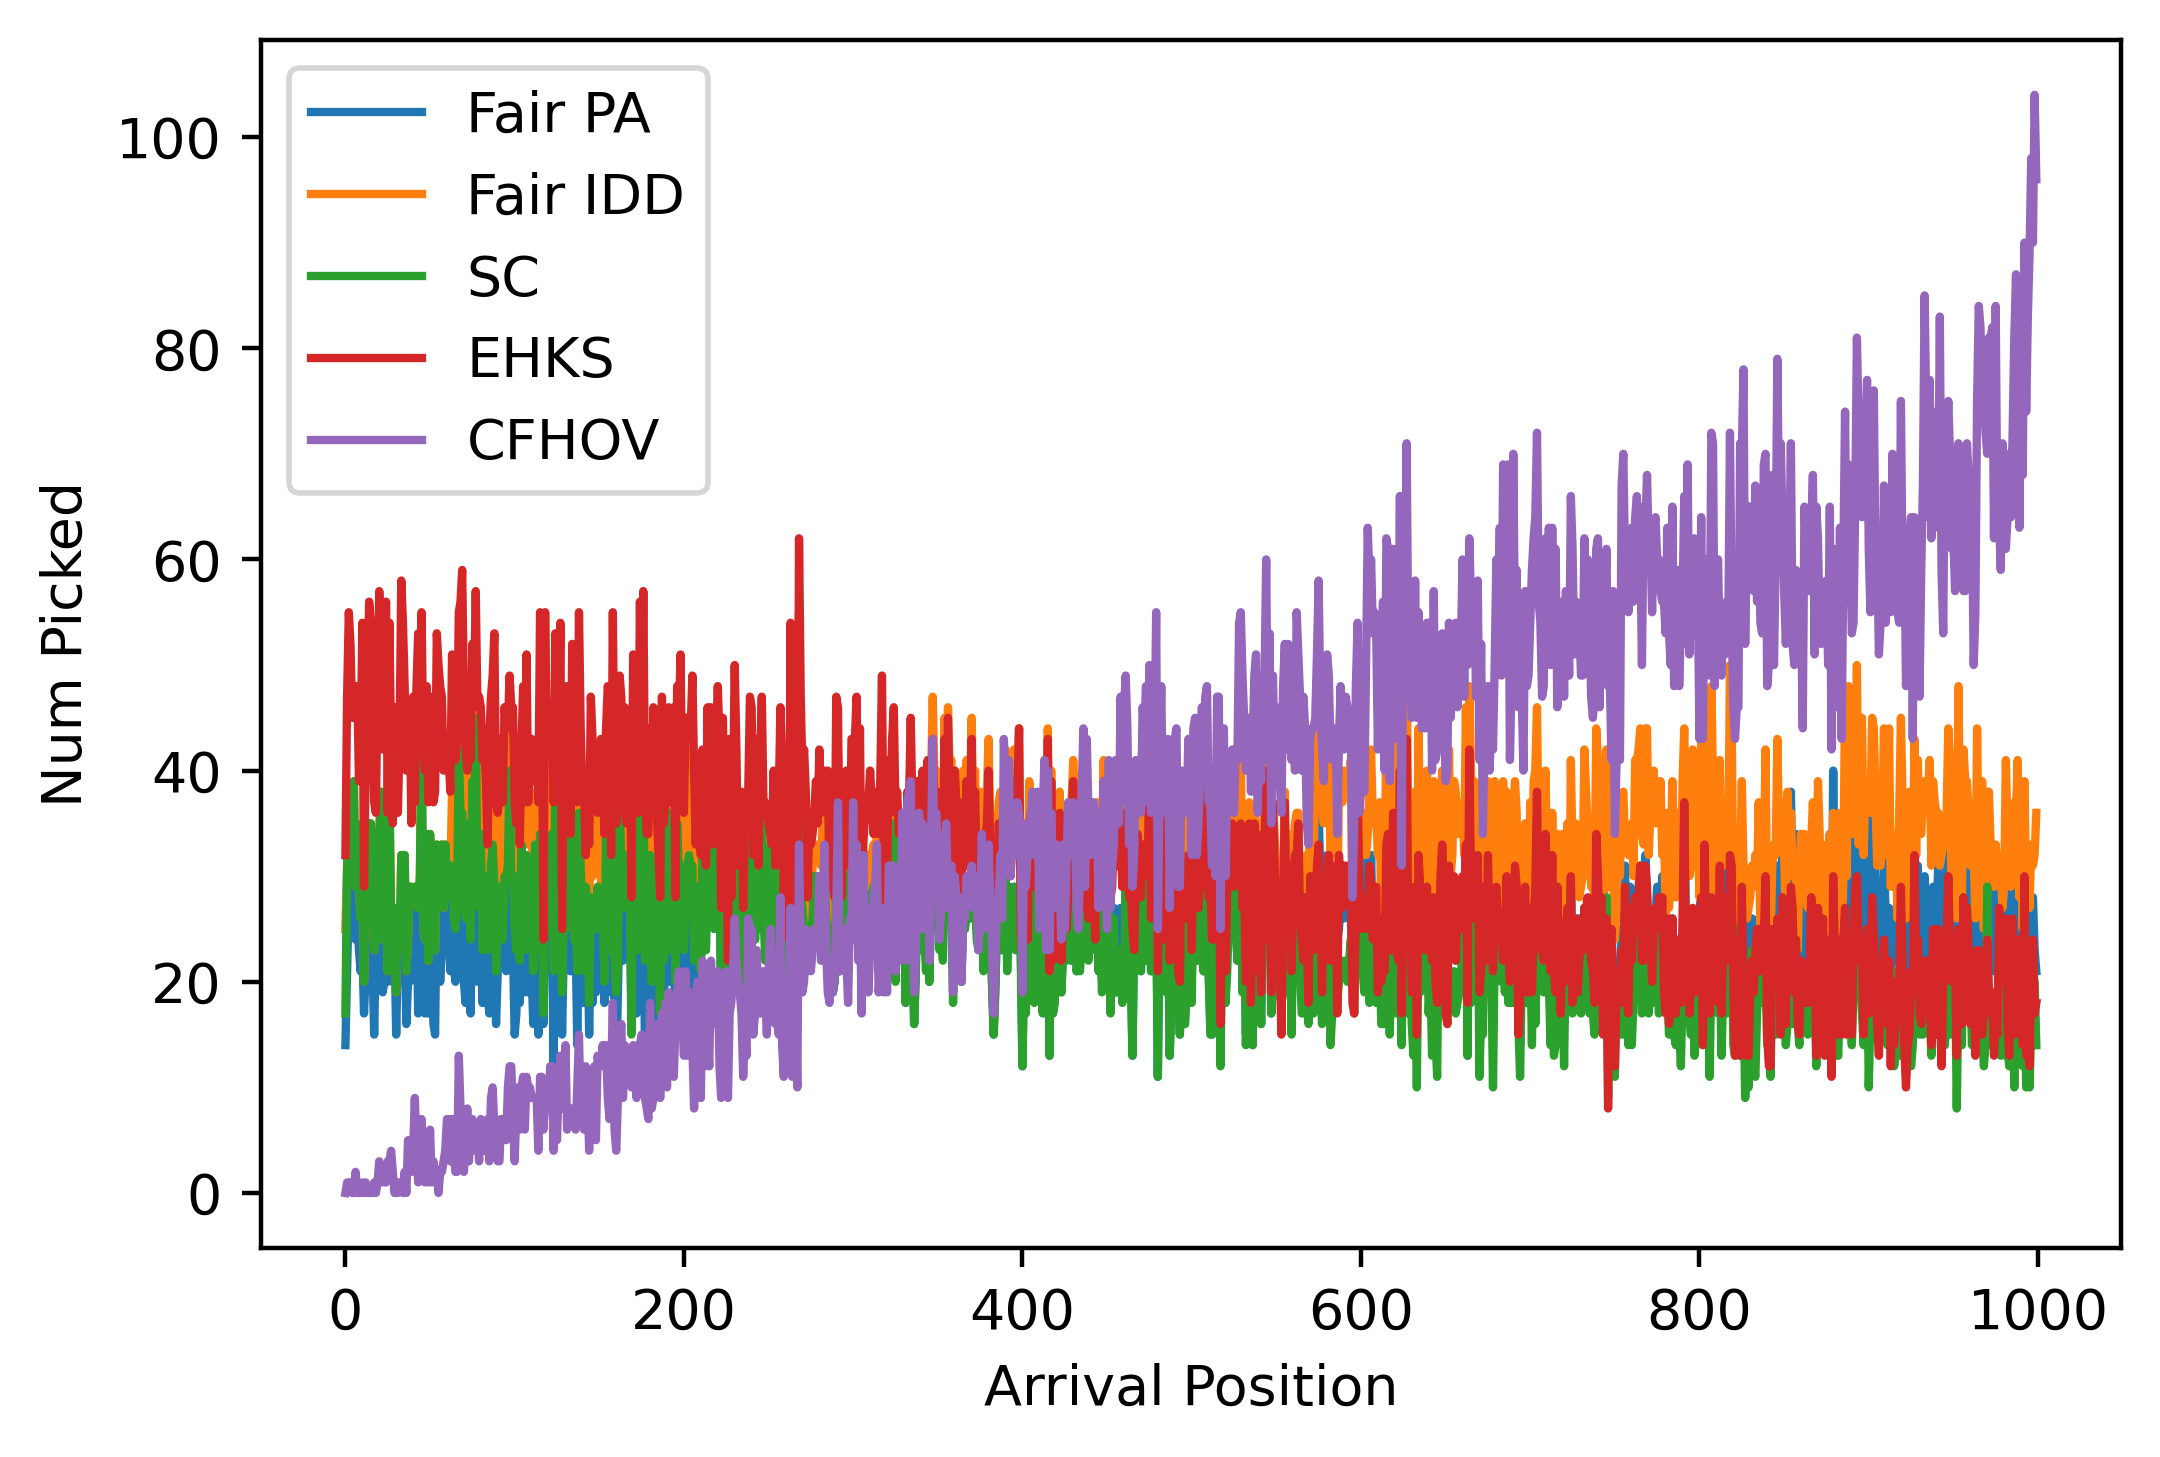
\includegraphics[width=1\textwidth]{media/Prophetplot_bi.png}
        \caption{Reproduced Binomial Distribution}
    \end{subfigure}
    \hfill
    \begin{subfigure}[b]{0.475\textwidth}
         \centering
    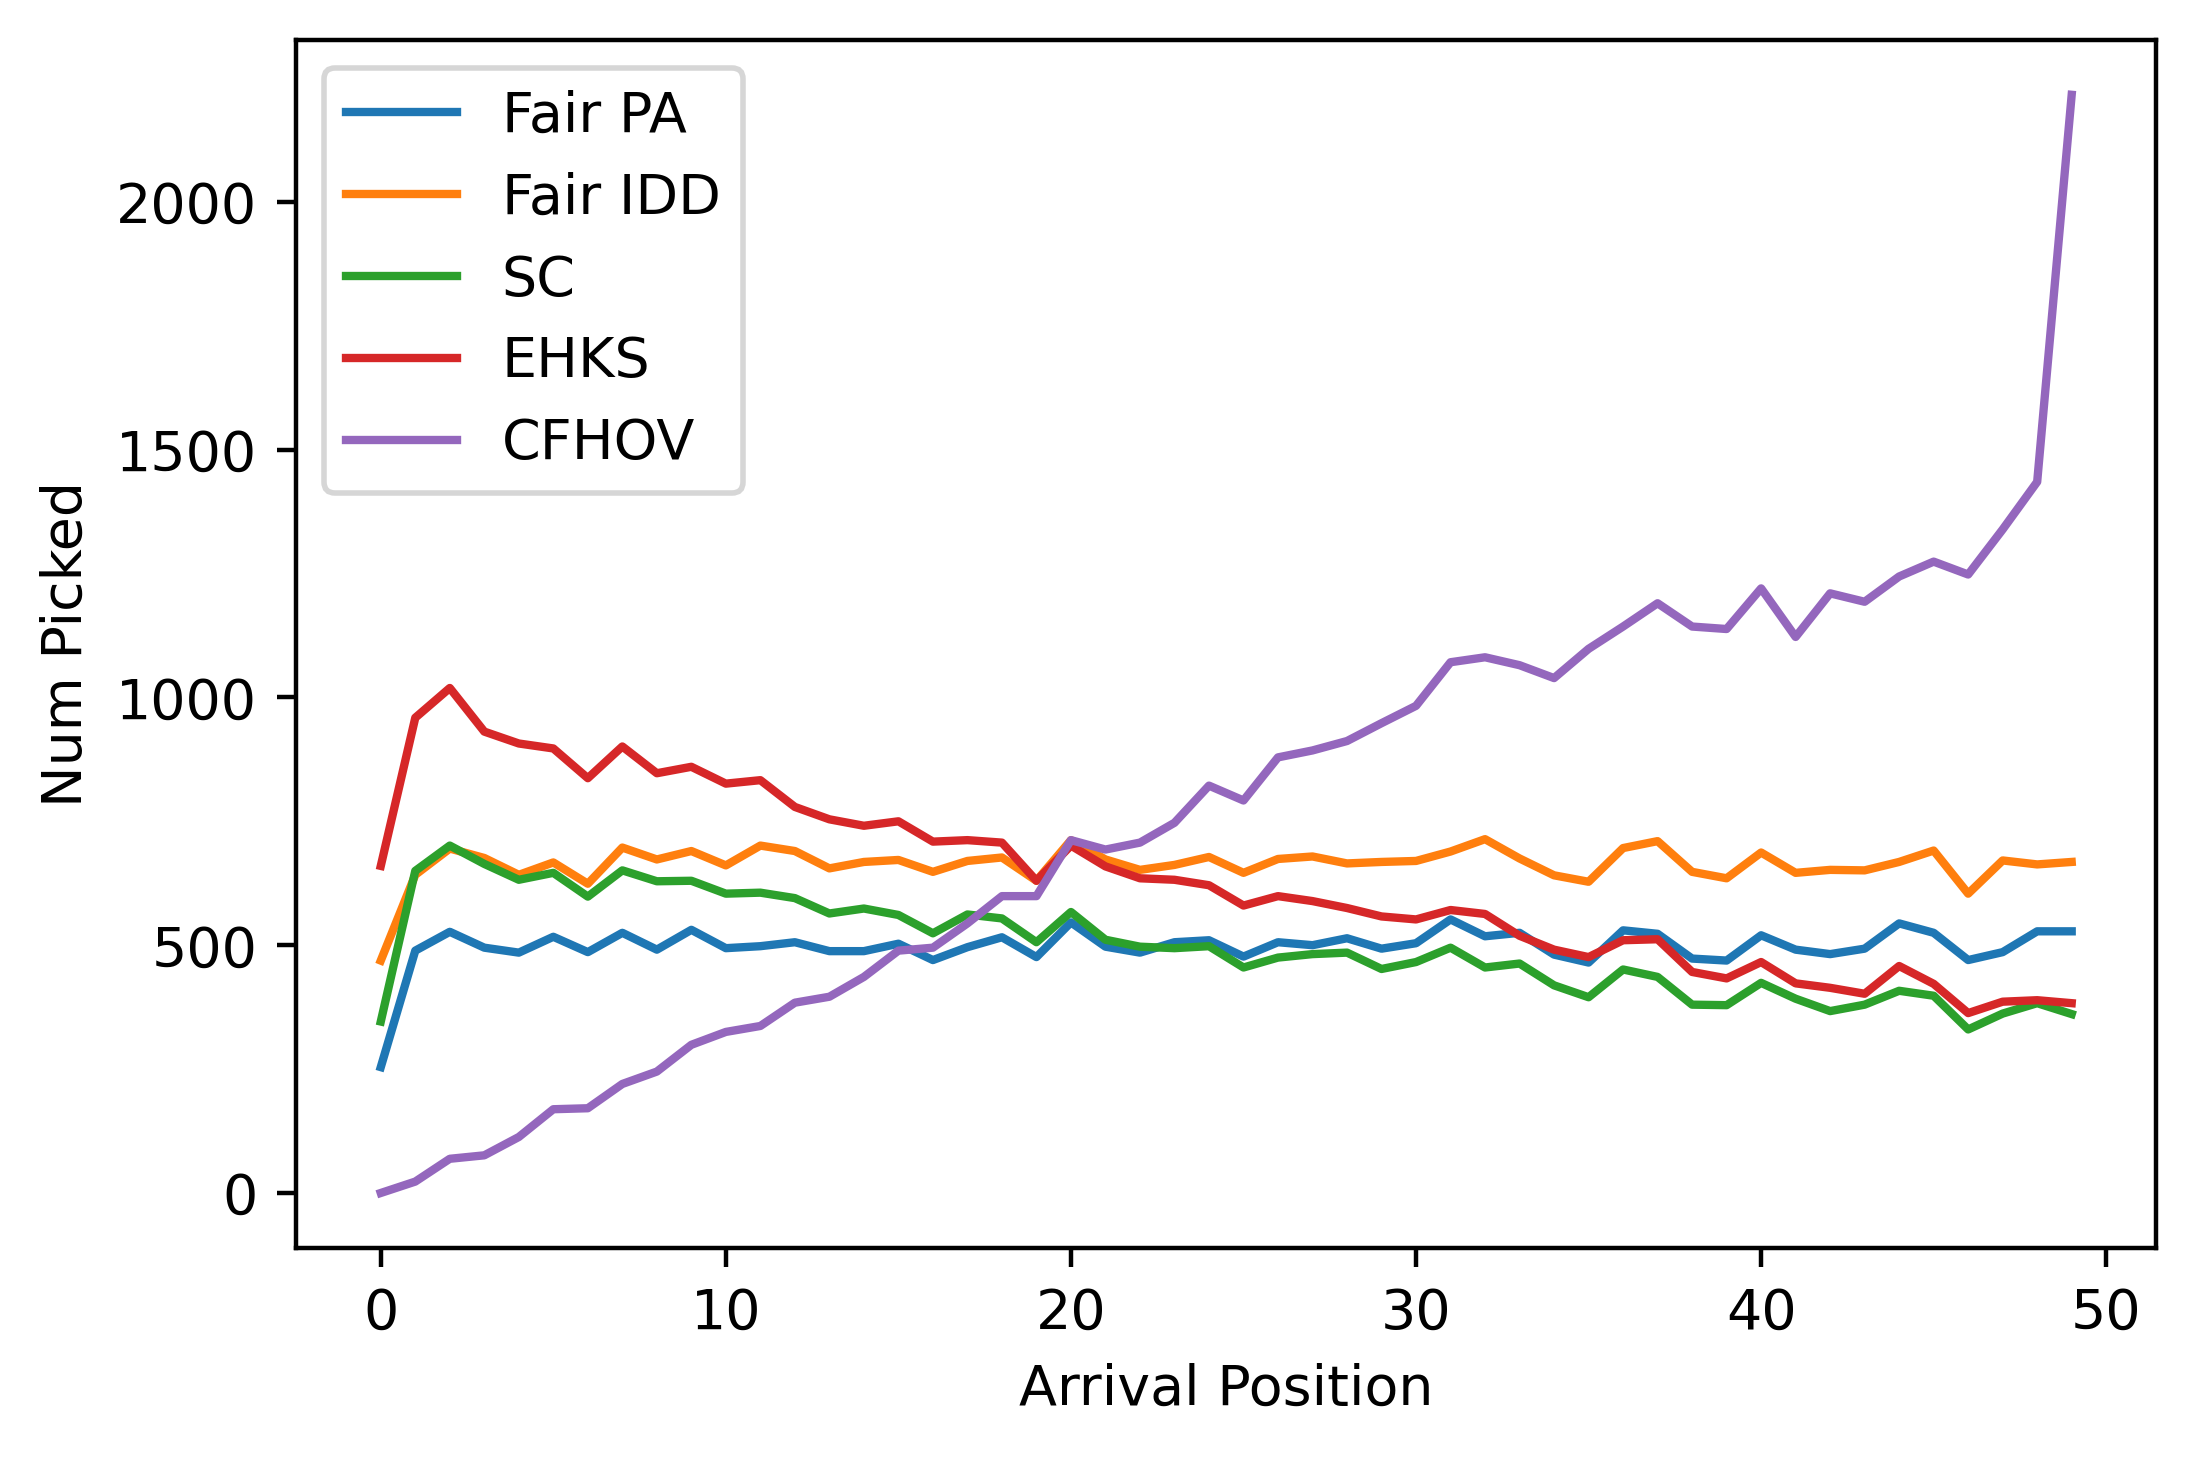
\includegraphics[width=1 \linewidth]{media/Prophetplot_unif.png}
    \caption{Reproduced Uniform Distribution}
    \end{subfigure}
    \caption{Reproduced results for the prophet experiments.}
    \label{fig:propresults}
\end{figure*}

\textbf{Extending to other data set (UFRGS) results}
\label{results_reproducting_original_paper}
\FloatBarrier
Figure \ref{fig:ufrgs_plot} shows the results of the experiments proposed in section \ref{Work_beyond_original_paper}. It can be noted that the pattern visible in the earlier secretary results still holds for a new, unequally distributed data set. However, when looking at Table \ref{tab:secretary}, a significant decrease in performance can be detected. The Bank and Pokec data sets scored +37.7\% and +36.8\% for F-Pick compared to S-Pick. The UFRGS only has an increase of +19.2\%. The difference is even more significant when comparing F-Max to S-Max; Pokec and Bank have an increase of +81.2\% and +81.0\%, UFRGS only has an improvement of +36.4\%. We can conclude that the performance increase of the Fair secretary algorithm is not as significant when using an unequally distributed data set, compared to the increase mentioned in the paper.
% However, when looking at Table \ref{tab:secretary}, it can be concluded that the Fair secretary algorithm performs significantly worse with this new data set compared to the SCSA algorithm.
\begin{figure}
    \centering
    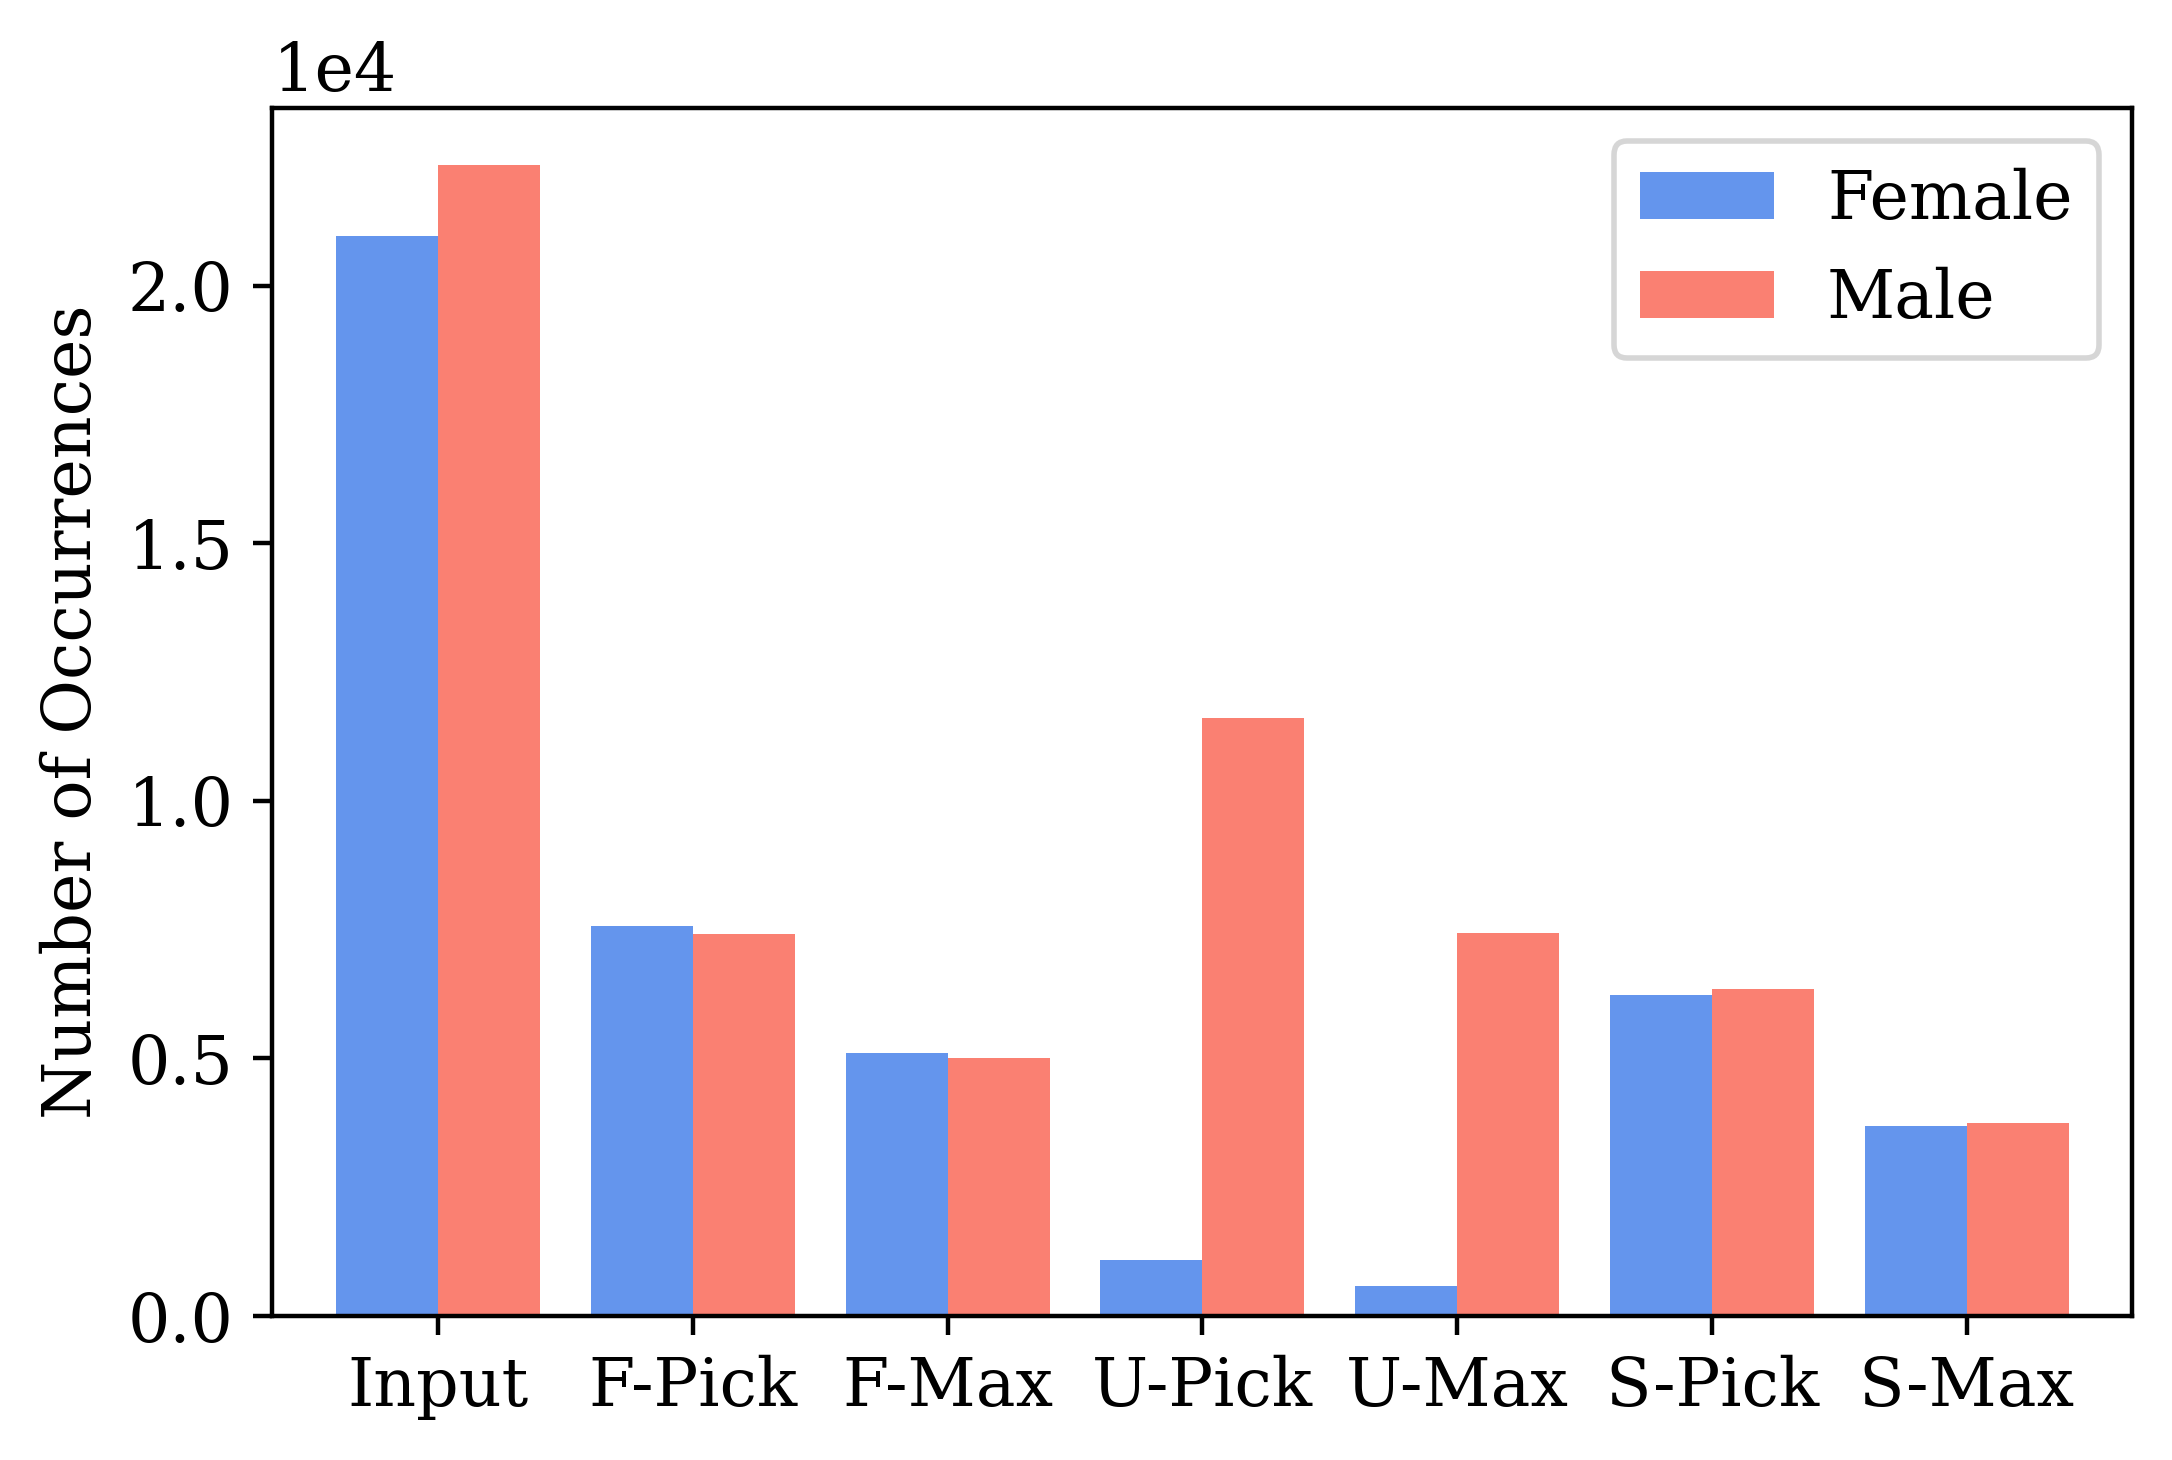
\includegraphics[width=0.5\linewidth]{media/Images_plots/Secretaryplot_ufrgs__.png}
    \caption{Secretary experiment applied to the UFRGS data set.}
    \label{fig:ufrgs_plot}
\end{figure}

% \newpage
\section{Discussion}
% Give your judgement on if your experimental results support the claims of the paper. Discuss the strengths and weaknesses of your approach - perhaps you didn't have time to run all the experiments, or perhaps you did additional experiments that further strengthened the claims in the paper.

In this research, we have tried to reproduce the work of \citep{correa2021fairness} as closely as possible. However, there are a few inconsistencies in the original code and paper, which caused complications. These points and our solution to them (if required) will be briefly discussed in the following paragraph.

Firstly, as mentioned before, the BMI thresholds for the pre-processing of the Pokec dataset were missing in the authors' work. This poses a problem as slight alterations to these thresholds yield different results. This problem was solved by finding concurring values in other research. Secondly, to limit the computation time of our reproduction, the size of the Pokec data set was limited from approximately 650.000 to 40.000 elements. The number of repetitions for this experiment was also decreased from 1.000.000 to 40.000. We opted for this solution as the distributions in the results did not change from these limits onward. Thirdly, the U-pick/U-max values in the secretary results of the original work are inconsistent due to randomness. It seems that changing the seed value of the random number generator in the \textit{C++} code heavily changes the output of the SA algorithm (U-pick/U-max). The SA results could therefore be cherry-picked as no further explanation was provided by the authors. Lastly, some inconsistencies are present in the paper. From minor typos e.g. using the word \textit{desbribed} instead of \textit{described}, to more serious mistakes, such as claiming that an increase of 1.721 is equal to (+73.1\%). A thorough reread of the paper would have resolved this.

\subsection{Reflection on our replication study}
The algorithms used in the original were clear and straightforward. The existing \textit{C++} code of the authors provided a good starting point for the verification of the results.

However, our goal was to further validate these claims and generalize them to a further extent. We did this by reproducing the work of the original paper. Reproducing the work efficiently in another language, in our case \textit{Python}, introduced some difficulties and took longer than expected. An execution of transliterated code resulted in an excessive run time. To tackle this problem, some of the data structures needed to be converted to \textit{NumPy} arrays to decrease computation time. This requires advanced knowledge of \textit{Numpy} and the use of data structures.

\subsection{Communication with original authors}
As certain parameters and split-off values were not clearly defined in either the paper or the original code, we reached out to the authors via mail to ensure a fair assessment of the reproduction. Examples of missing split-off values are the BMI category thresholds for the pre-processing of the Pokec data set. These category values are not fixed in literature and differ depending on age and nationality. At the time of writing this report, we had not yet heard back from the authors. We resolved this by assuming certain values and explanations, which are all documented in our paper.
